%\documentstyle[epsf,twocolumn]{jarticle}       %LaTeX2.09仕様
%\documentclass[twocolumn]{jarticle}     %pLaTeX2e仕様
\documentclass{jarticle}     %pLaTeX2e仕様

\setlength{\topmargin}{-45pt}
%\setlength{\oddsidemargin}{0cm} 
\setlength{\oddsidemargin}{-7.5mm}
%\setlength{\evensidemargin}{0cm} 
\setlength{\textheight}{24.1cm}
%setlength{\textheight}{25cm} 
\setlength{\textwidth}{17.4cm}
%\setlength{\textwidth}{172mm} 
\setlength{\columnsep}{11mm}

\kanjiskip=.07zw plus.5pt minus.5pt

\usepackage{graphicx}
\usepackage[dvipdfmx]{color}
\usepackage{subcaption}
\usepackage{enumerate}
\usepackage{comment}
\usepackage{url}
\usepackage{multirow}
\usepackage{diagbox}
\usepackage{bm}
\usepackage{amssymb}
\usepackage{amsfonts}
\usepackage{booktabs}



\begin{document}
  \noindent
  \onecolumn
  \hspace{1em}

  情報工学英語演習
  \hfill
  \ \  学籍番号1201201100 西村昭賢 

  \vspace{2mm}
  \hrule
  \begin{center}
  {\Large \bf AttentionIsAllYouNeedの和訳}
  \end{center}
  \hrule
  \vspace{3mm}

\section*{Authors}
Ashish Vaswani, Noam Shazeer, Niki Parmar, Jakob Uszkoreit, Llion Jones, Aiden N.Gomez, Lukasz Kaizer, Illia Polosukhin\cite{Transformer}

\section*{Abstruct}
今までの主要な系列変換モデルは,エンコーダとデコーダを含む
複雑な RNN や CNN に基づいていた.最も良いパフォーマンスであったモデルも,エンコーダとデコーダを注意機構で接続しているモデルであった.\par
私達は, RNN や CNN を用いず,注意機構のみからなる Transformer と呼ばれる新しい簡潔なモデルを提案する. 2 回の翻訳実験の結果, Transformer は今までのモデルより優れており,更には,より並列化が可能で学習の時間も少ないことが分かった.
Transformer は WMT2014 英独翻訳タスクにおいて,「プロの翻訳者の訳と近ければ近いほどその機械翻訳の精度は高い」という考え方に基づく機械翻訳の評価方法である BLEU スコア\cite{BLEU}で 28.4BLEU を記録した.これは,複数のモデルを融合させて 1 つの学習モデルを生成するアンサンブル学習\cite{ensemble}を含めたこれまでの最高記録を 2BLEU 上回る結果であった.また, WMT2014 英仏翻訳タスクにおいては, 8 個の GPU を用いた 3日半の学習というこれまでの最先端のモデルの学習よりも遥かに少ない学習コストで, 41.0BLEU という単一モデルでの最高記録を打ち立てた.

%sequence transduction model=系列変換モデル とした


\section{Introduction}
RNN, 特に RNN において文章の長期的な依存関係を学習できるようにした LSTM\cite{LSTM} やgated RNN \cite{GRU} は,言語モデルや機械翻訳などの系列変換問題への最適な手法として確固たる地位を築いていた.
それ以来, RNN とエンコーダー-デコーダー構造の限界を押し上げる数々の努力がなされてきた.
\par
RNN では,通常,入力と出力の時系列データの時間的な位置に沿って計算する.
計算は逐次的に行われ,時刻 $t$ における隠れ状態 $h_\mathrm{t}$ は,時刻 $t-1$ の隠れ状態の $h_\mathrm{t-1}$ と時刻 $t$ における入力から導かれる.
このように本質的に逐次的な性質を孕んでいるため,学習の並列処理が困難である.そのため,メモリの制約上,長い系列データなどの学習には致命的であった.
直近の研究ではfactorization tricksやconditional computationといった方法で計算効率がかなり改善され,後者ではモデルの性能まで向上させることができたが,逐次的な計算の問題は残ったままだった.\par
注意機構は入力と出力の系列データにおける距離を気にせず依存関係をモデル化することができ,様々なタスクにおいて有効な系列変換モデルにおける必要不可欠な部分となっている.しかし,一部の場合には注意機構は RNN と組み合わせて用いられる.\par
本研究で私達が提案する Transformer は, RNN を用いず,注意機構のみで入力と出力の完全な依存関係を取り出すモデルのアーキテクチャである.
 Transformer は学習の並列処理が可能であり, 8 個の P100 GPU で 12 時間という小規模な学習後に,過去最高の機械翻訳性能に達することができた.


\section{BackGround}
逐次的な計算を減らすという目標は, Extended Neural GPU, ByteNet, ConvS2S といったモデルの基礎にもなっている.これらはどれも CNN を基本構成要素として,入力と出力のすべての位置で隠れ状態の値を計算する.これらのモデルにおいて,任意の入力の位置と出力の位置の信号を関連付けるために必要な計算時間は, ConvS2Sd では線形的, ByteNet では指数的に増加する.
そのため離れた位置の依存関係を学習することはより困難になる.
 Transformer では,この処理を定数時間で計算できる.注意機構で重み付けした位置を平均化することで入力データに対する有効な解像度が下がってしまうが, 3.2 節で述べる多頭注意により相殺できる.\par

内部注意とも呼ばれる自己注意は,単一系列内の異なる位置を参照し,類似度で重み付けを行うことで系列要素を関連付ける注意機構である.自己注意は文章読解,要約,テキスト含意,独立した文の表現の学習などのタスクで用いられ成功している.\par

End-to-End memory Networks は RNN の代わりに再帰的な Attention を元にしており,単純な言語の質疑応答,言語モデリングといったタスクにおいて優れた結果を示している.\par

しかし私達が知る限り, Transformer は 入出力の表現を計算する際に, RNN や CNN を用いずに, 自己注意のみに依存した最初の系列変換モデルである.次節以降では,Transformer,自己注意について説明しこれまでのモデルと比較した利点を議論する.




\section{Model Architecture}
優位性のある系列変換モデルはエンコーダ-デコーダ構造を有している.エンコーダは配列で表現される入力 ($x_\mathrm{1}$,...,$x_\mathrm{n}$) を配列 \bm{$z$}=($z_\mathrm{1}$,...,$z_\mathrm{n}$) に変換する.
デコーダは \bm{$z$} から出力として配列 ($y_\mathrm{1}$,...,$y_\mathrm{n}$) を 1 要素ずつ出力する.
このステップで,このモデルは,新しく生成する要素はこれまでに生成した要素のみに依存する自己回帰モデル\cite{自己回帰モデル}であり,直前に生成された要素を新しく入力として次の要素を生成する.\par
Transformer は図 1 に示すように,全体としてはエンコーダ-デコーダ構造を踏襲しつつ,自己注意層と point-wise 全結合層を積み重ねた層を使用している.

\begin{figure}[ht]
  \centering
  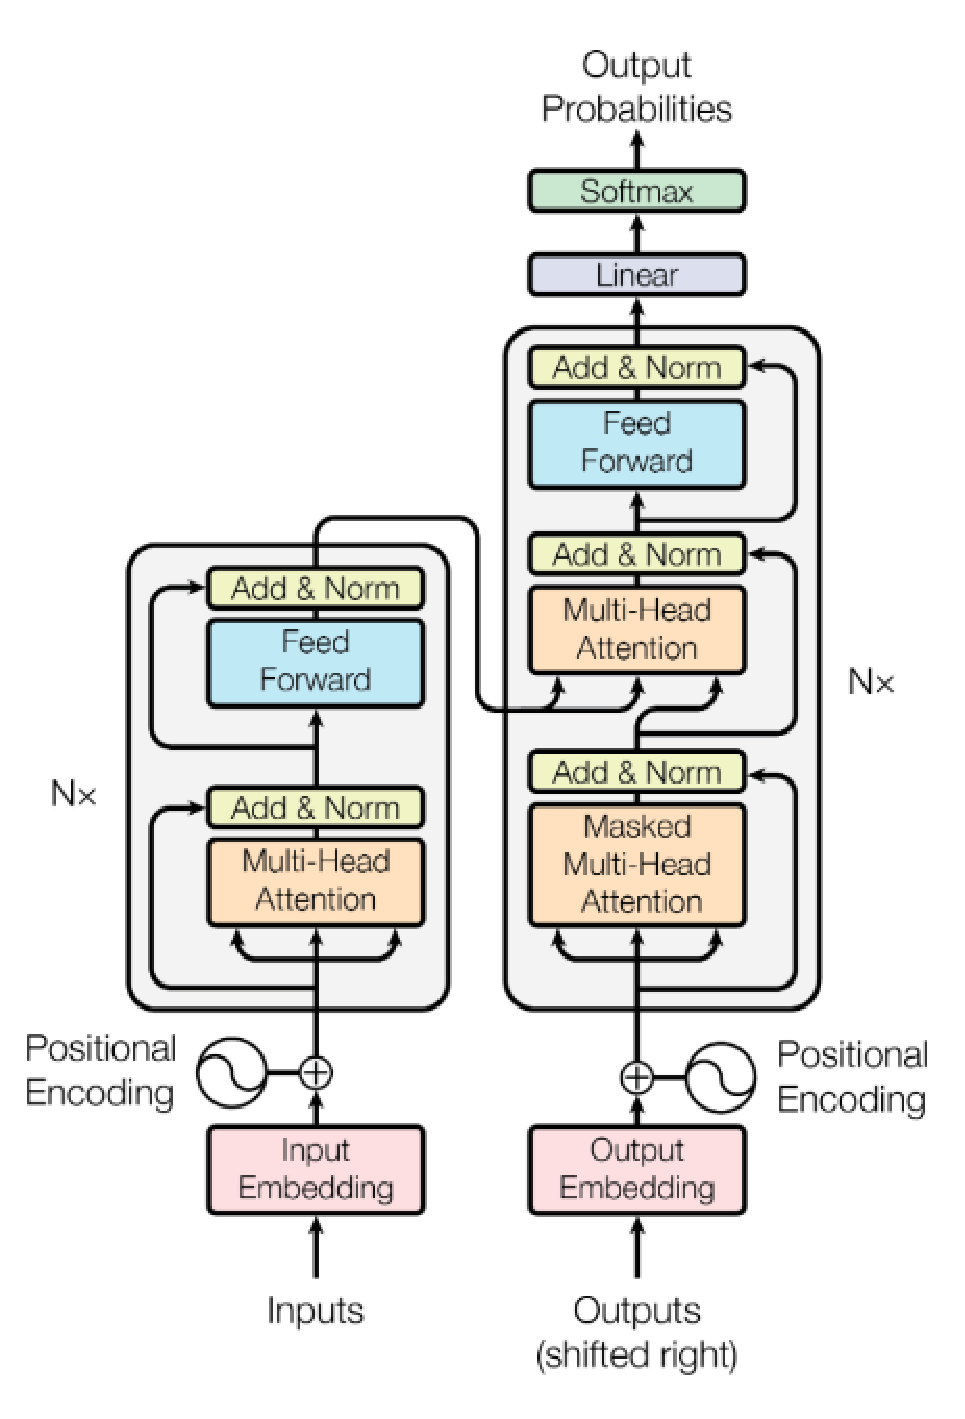
\includegraphics[width=100mm]{assets/Figure1.eps}
  \caption{ Transformer のモデルアーキテクチャ.}
  \label{Figure1}
\end{figure}


\subsection{Encoder and Decoder Stacks}
\textbf{エンコーダ}: 6 層からなり,各層は全く同じ構造である.それぞれの層は 2 つの下位層を持ち,下位層の後には残差接続と標準化が行われている.
よって,入力を $x$ , 下位層自身の出力を Sublayer($x$) として, 残差接続では $x+$Sublayer($x$) ,下位層全体としての出力は LayerNorm($x$+Sublayer($x$)) となる\cite{残差接続}.残差接続を容易にするために,すべての下位層, 埋め込み層は,出力の次元を $d_\mathrm{model}=512$としている.\par
\par
\textbf{デコーダ}: デコーダも同一の 6 層からなる.エンコーダの持つ 2 つの下位層に加えて,エンコーダの出力を入力として受ける 3 つ目の下位層を加えている.エンコーダと同じく,下位層の後には残差接続や標準化が行われている.ただ, 自己注意層はエンコーダ層とは異なり,後続の要素を参照しないようにしている.このマスキングと,出力が 1 要素ごとnに補われていくことを組み合わせることで,マスキングにより地点 $i$ での予測が地点 $i$ 未満での既知の出力のみに依存することが保証される.

\subsection{Attention}
注意機構はクエリとキーとキー値のセットを出力へマッピングする機構である.ここで,クエリやキー,キー値,出力はすべてベクトルである.出力はキー値の重み付き和として計算され,それぞれのキー値への重みはクエリとクエリに対応するキーからの変換関数で計算される.

\subsubsection{Scaled Dot-Product Attention}
本研究で独自に考案した注意機構を"標準化内積注意"と呼ぶ.図2に標準化内積注意のアーキテクチャを示す.\par

\begin{figure}[ht]
  \centering
  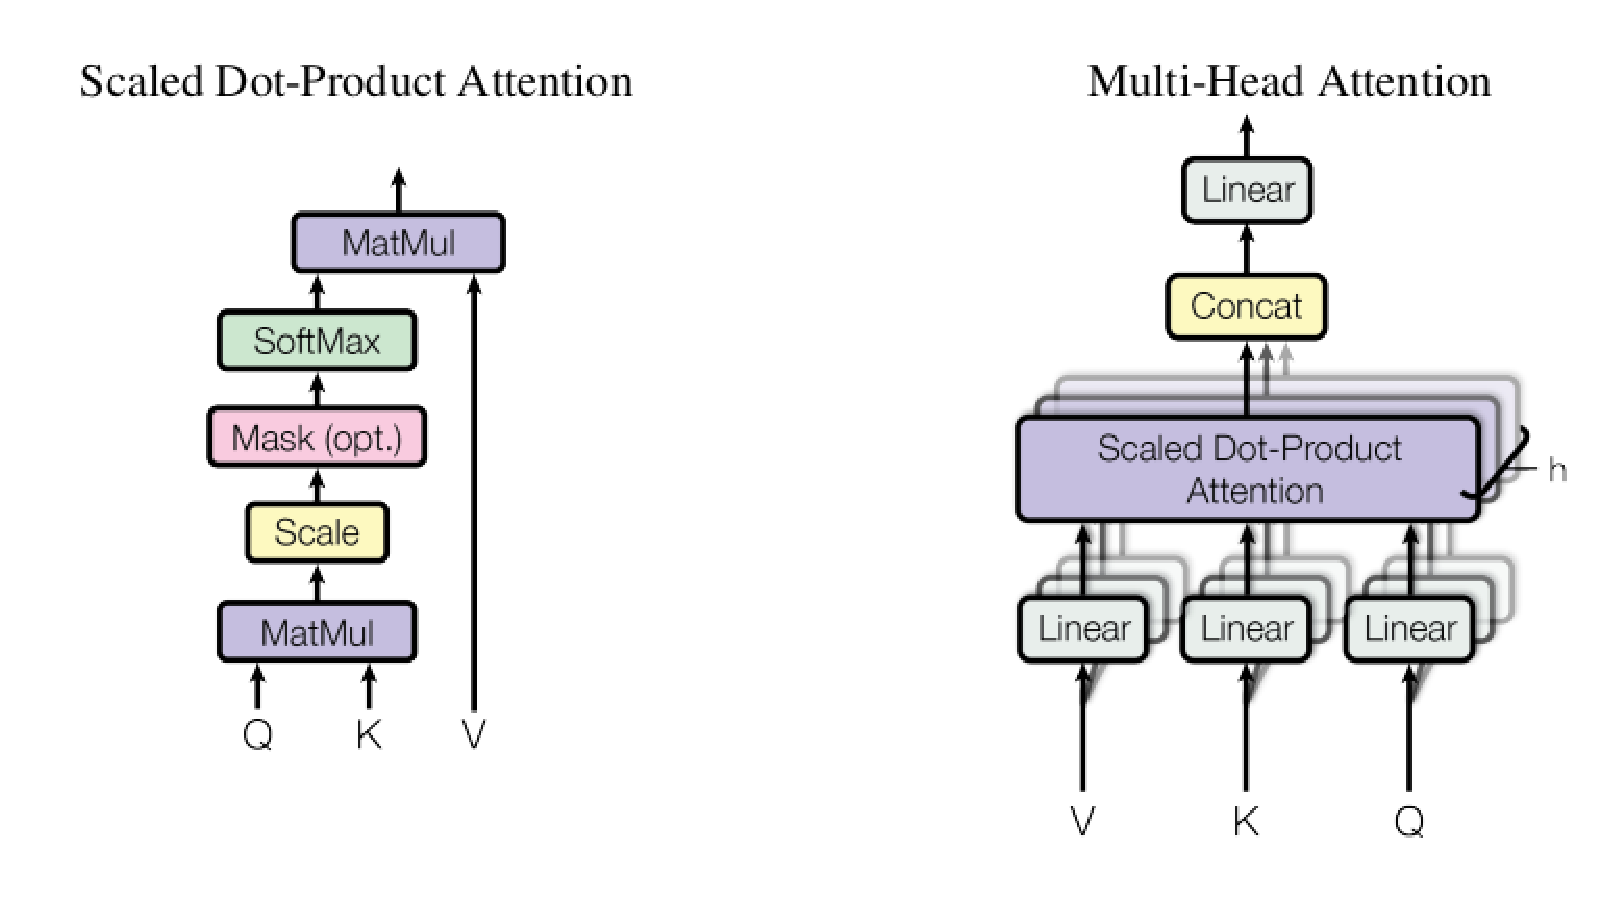
\includegraphics[width=100mm]{assets/Figure2.eps}

  \caption{(左)標準化内積注意. (右)複数の注意機構層が並列に構成されている多頭注意.}
  \label{Figure2}
\end{figure}


入力はクエリと次元$d_\mathrm{k}$のキー,次元$d_\mathrm{v}$のキー値からなる.クエリとキーの内積を計算し,それを$\sqrt{d_\mathrm{k}}$で割り,softmax関数を適用しキー値の重みを得る.
実際にはクエリ,キーやキー値を行列 $Q$, $K$, $V$にまとめて計算している.行列による注意機構の出力は(1)式のように表せる.

\begin{equation}
  \mathrm{Attention}(Q,K,V) = \mathrm{softmax}(\frac{QK^T}{\sqrt{d_\mathrm{k}}})V
\end{equation}

\par

最も一般的に利用される注意機構としては加法注意と内積注意の2つがある.内積注意は,標準化内積注意から $\sqrt{d_\mathrm{k}}$ で割る処理を除いたものである.加法注意は一つの隠れ層を持つ feed-forward network を用いて変換関数を計算している.2つの注意機構は理論的には似ているが,高度に最適化された行列積のコードを内包しているため内積注意のほうが計算が遥かに早く,メモリ効率も良い.\par
$d_\mathrm{k}$ が小さい値である時はこの 2 つの注意機構は同様に作用するが, $d_\mathrm{k}$ が大きい値である時には,加法注意は標準化をしない内積注意より性能が良くなる. 標準化内積注意では, $d_\mathrm{k}$ が大きい値である時に,内積の値が急激に増加し, softmax 関数の勾配消失が起こると考え,それを防ぐために内積を $\frac{1}{\sqrt{d_\mathrm{k}}}$ で標準化している.

\subsubsection{Multi-Head Attention}
次元 $d_\mathrm{model}$ におけるキーとキー値とクエリを用いた単一の注意関数を使用する代わりに,クエリとキーとキー値に $h$ 回それぞれ異なる変換が学習されている線形変換をし,次元を $d_\mathrm{k}$, $d_\mathrm{k}$, $d_\mathrm{v}$にそれぞれ削減したほうが都合が良いと判明した.
射影したクエリ,キー,キー値それぞれに対して,注意関数を並列に実行し,次元 $d_\mathrm{v}$ の出力を得る.それらを Concat 層で連結し,もう一度線形射影して最終的な出力を得る.図 2 にこの一連の過程を示す.
\par
多頭注意により,異なる要素の異なる部分ベクトル空間を見ることができ,結果として表現力が高まる.\cite{Multihead}単頭注意では,このようなことはできない.
\par

\begin{eqnarray*}
  \mathrm{MultiHead}(Q,K,V)&  = & \mathrm{Concat}(head_\mathrm{1},...,head_\mathrm{h})W^O   \\
  ここで, head_\mathrm{i} & = & \mathrm{Attention}(QW_\mathrm{i}^Q,KW_\mathrm{i}^K,VW_\mathrm{i}^V)
\end{eqnarray*}

射影関数のパラメータの行列は,
$W_\mathrm{i}^Q \in \mathbb{R} ^ {{d_\mathrm{model}} \times {d_\mathrm{k}}}$,
$W_\mathrm{i}^K \in \mathbb{R} ^ {{d_\mathrm{model}} \times {d_\mathrm{k}}}$,
$W_\mathrm{i}^V \in \mathbb{R} ^ {{d_\mathrm{model}} \times {d_\mathrm{v}}}$と\par
$W_\mathrm{i}^O \in \mathbb{R} ^ {{hd_\mathrm{v}} \times {d_\mathrm{model}}}$である.

本研究では, $h=8$ の並列の標準化内積注意層を用いて,次元を
 $d_\mathrm{k} = d_\mathrm{v} = d_\mathrm{model}/h = 64$ とした.
次元の削減により,総計算コストを,次元の削減を行わなかった場合の単頭注意と同等まで削減することができた.

\subsubsection{Applications of Attention in our Model}
Transformer では,多頭注意を以下の 3 つの方法で採用している.
\begin{itemize}
  \item "エンコーダ-デコーダ注意層"では,クエリはデコーダにおける直前の層から生まれ,キーとキー値はエンコーダの出力から生まれる.デコーダ内のすべての要素が入力文のすべての要素を見ることができる.すなわち系列間のトークン表現間で注意処理を行う.これは, seq2seq モデルの典型的なエンコーダ-デコーダ注意機構を模倣している.
  \item エンコーダにおける自己注意層では,キー,キー値,クエリの全てが,一つ前のエンコーダ層の出力から生まれている.エンコーダ内の系列内のそれぞれの要素は,エンコーダの一つ前の層の出力の系列内の全ての要素を参照することができる.
  \item 同様に,デコーダ内の自己注意層も,デコーダの全層の要素を参照することができるが,自動回帰的な特性を保持するために,左向きへの情報の流出を防がなければならない.すなわち,翻訳済の単語に影響が出ないようにしなければ行けない.本研究では標準化内積注意の中で,不当な接続に相当する部分を-$\infty$にマスキングして, softmax 層の入力として与えることで,これを実現している.図 2 にこの過程を示している.
\end{itemize}

\subsection{Position-wise Feed-Forward Networks}
注意層に加えて,エンコーダとデコーダ内のそれぞれの層には,完全に連結した feed-forward network が含まれている. feed-forward network は,2つの線形変換の間に ReLU 関数を適用した形となっている.

\begin{equation}
  \mathrm{FFN}(x) = \mathrm{max}(0,xW_\mathrm{1}+b_\mathrm{1})W_\mathrm{2} + b_\mathrm{2}
\end{equation}

線形変換は入力の異なる要素に対しても同じ値を掛けるのに対して,線形層ごとに異なる値のパラメータを用いる.言い換えると,カーネルサイズが 1 の 2 つの畳み込みとして捉えることができる.
入出力の次元は $d_\mathrm{model} = 512$ とし, feed-forward network 内では次元は $d_\mathrm{ff} = 2048$ としている.

\subsection{Embeddings and Softmax}
他の系列変換モデルと同様に,学習済みの埋め込み層を用いて入力と出力のトークンを次元 $d_\mathrm{model}$ のベクトルに変換する.また,一般的な学習済みの線形変換と softmax 関数を用いて,デコーダの出力を予測済みのトークンの確率に変換している. Transformer は, 2 つの埋め込み層と softmax 層の前の線形変換で同じ重み行列を使用している.また,埋め込み層では $\sqrt{d_\mathrm{model}}$ を掛けている.

\subsection{Positional Encoding}
私達のモデルは RNN や CNN を含んでいないため,モデルが系列内の要素の順番を利用するために,絶対的であれ,相対的であれ何らかの要素の順番の情報を定義する必要があった.結果として, "positional encoder" を入力の埋め込み層に付け加え,エンコーダとデコーダの最下層に入れることとした.埋め込み層との加算を行うために, positional encoding の次元は埋め込みそうと同じ $d_\mathrm{model}$ とした.\par
本研究では, positional encoding として別々の周波数を持つ sin 関数, cos 関数を用いた.

\begin{eqnarray*}
  PE_{(pos,2i)} &= &sin(pos/10000^{2i/d_\mathrm{model}}) \\
  PE_{(pos,2i+1)} &= &cos(pos/10000^{2i/d_\mathrm{model}})
\end{eqnarray*}

ここで, $pos$ は要素の位置, $i$ は次元である.つまり, position encoding のそれぞれの次元は正弦波に該当する.波長は $2\pi$ から $10000・2\pi$ まで段階的に増加していく.この関数を採用した理由は,モデルが系列の要素の相対的な位置を簡単に学習できると仮説を立てたためである.なぜなら,任意の定数オフセット $k$ において, $PE_{pos+k}$ は $PE_{pos}$ の線形関数として表すことができるからだ.\par
別の論文の学習済みの positional embedding を用いた実験をしたところ,本論文と別論文の結果はほぼ等しくなった.そこで,本研究の正弦波を用いた方法が学習時よりもより長いデータに対しても対応できると判断し採用した.


\section{Why Self-Attention}

本章では,self-attention層における様々な側面を,RNNやCNNと比較する.RNNやCNNは可変長の配列
($x_\mathrm{1}$,...,$x_\mathrm{n}$)を,同じ長さの配列($z_\mathrm{1}$,...,$z_\mathrm{n}$)に変換し,エンコーダーやデコーダーなどの典型的なsequence transductionの隠れ層に用いられる.私達がself-attentionを使う理由としては,3つの大きな不足を感じる物事があったからである.
\par
1つ目は層ごとの計算の複雑さである.2つ目は本来並列化が可能な計算量である.これは必要最低限の配列計算量から算出できる.
\par
3つ目がモデルのネットワークで遠い位置関係の要素の依存関係を認識できる経路の長さである.
遠い位置関係の要素の依存関係を学習することは,多くのsequence transductionタスクにおいて重要な課題である.そのような依存関係を学習するための1つの重要な要因は順方向か逆方向かの信号がネットワークを通る経路の長さである.入力と出力の位置関係の間の経路が短ければ短いほど,より長い位置関係での依存関係の学習が容易になる.従って,私達は異なる種類の層からなるネットワークにおいての入力と出力の位置間の最大の経路長を比較した.表1にその結果を示す.

\begin{table}[hbtp]
  \caption{異なる種類の層における層ごとの計算の複雑さ,配列計算の計算量,最大経路長.$n$は配列の長さ,$d$は表現の次元,$k$はCNNのカーネルのサイズ,$r$は制限付きSeld-Attentionの近傍サイズ.}
  \label{table:path length}
  \small
  \centering
  \scalebox{1.2}[1.2]{
    \begin{tabular}{lccc}
      \hline
      Layer Type  & Complexity per Layer  &  Sequential Operations & Maximum Path Length \\
      \hline 
      Self-Attention  & $O(n^2・d)$  & $O(1)$ & $O(1)$ \\
      Recurrent  & $O(n・d^2)$   & $O(n)$ & $O(n)$ \\
      Convolutional  & $O(k・n・d^2)$  & $O(1)$ & $O(log_k(n))$ \\
      Self-Attentional(restricted)  &  $O(r・n・d)$  &  $O(1)$ & $O(n/r)$ \\
      \hline
    \end{tabular}
  }
  
\end{table}

表1で示した通り,配列計算にRNNが$O(n)$時間かかるのに対して,Self-Attentionは$O(1)$時間,すなわち定数時間で行うことができる.計算の複雑さという観点では,一般的に機械翻訳での文の表現では$n<d$であることから,Self-AttentionはRNNより優れていると言える.
非常に長い文章に関するタスクに関して計算のパフォーマンスを向上させるためには,それぞれの予測に対応する入力文のサイズ$r$の範囲しか考えないという制限をSelf-Attentionに課す方法がある.しかし,この方法では,最大経路長が$O(n/r)$となってしまう問題がある.これは将来の研究の課題である.
\par
カーネルのサイズ$k$が,$k<n$となるような1層のCNNは,入力と出力の全てのペアを関連付けることはできない.そうするためには,連続したカーネルの場合は$O(n/k)$の積み重なった畳み込み層が必要,膨張畳込みの場合でも$O(log_k(n))$の層が必要となる.このため,最大経路長が増えてしまう問題が生じる.CNN層は,カーネルのサイズ$k$により,一般的にRNN層よりも計算が複雑になる.しかし,Separable convolutionsは計算の複雑さを$O(k・n・d + n・d^2)$まで減らしている.$k=n$の場合,Separable convolutionsは本研究で採用しているself-attention層とpoint-wise feed-forward network層の組み合わせと計算の複雑さは等しくなる.
\par
良い面として,self-attentionはより解釈しやすいモデルを得ることができる.モデルのattention分布について,付録で例を示して議論する.Attentionはそれぞれのタスクをきちんと学習するだけでなく,文の構文規則や意味構造になぞらえた振る舞いをしているようだ.

\section{Training}
本章では,私達のモデルの学習計画について記載する.

\subsection{Training Data and Batching}
英独翻訳に関して,450万もの文からなるstanderd WMT 2014 English-Germanデータセットを用いて学習を行った.文はbyte-pair encodingでエンコードされており,約37,000個のトークンの語彙が共有されている.英仏翻訳では,3600万もの文からなる大規模なWMT 2014 English-Frenchデータセットを用いた.トークンを32,000個の語彙に分割して使用した.文のペアはおおよその文の長さでバッチ処理を行った.それぞれの学習用バッチは文章対がまとまっており,おおよそ25,000個のsource token,target tokenが含まれる.

\subsection{Hardware and Schedule}
モデルの学習は,8個のNVIDIA P100 GPUを搭載した1つの計算機で行った.
本論文で述べたハイパーパラメータを使ったベースモデルでは,訓練の1ステップあたり0.4秒かかった.ベースモデルは100000ステップの合計で12時間学習を行った.大きいモデルでは1ステップあたり1.0秒かかり,300000ステップ,計3.5日かかった.

\subsection{Optimizer}
optimizerとしてAdamを用いた.パラメータは$\beta_\mathrm{1} = 0.9$,$\beta_\mathrm{2} = 0.98$, $\epsilon = 10^{-9}$とした.学習率は学習を行うに従って以下の式に応じて変更した.

\begin{equation}
  lrate = d_\mathrm{model}^{-0.5}・\mathrm{min}(step\_num^{-0.5},step\_num・warmup\_steps^{-1.5})
\end{equation}

学習の際,学習率は$warmup\_step$まで線形的に増えていくが,それ以降のステップでは,ステップ数の平方根の逆数に比例して減少していく.

\subsection{Regularization}
実験の際,3つの正則化を採用した.

\textbf{Residual Dropout}
それぞれの下位層の出力が残差接続される前にDropout処理を行った.それに加えて,エンコーダーとデコーダー両方のembeddingsとpositional encodingの和にもDropout処理を行った.ベースモデルでは,$P_{drop} = 0.1$とした.

\textbf{Label Smoothing}
学習中,$\epsilon_{ls} = 0.1$としてLabel Smoothingを行った.モデルが曖昧さを学ぶことで,翻訳の正確さの指標であるperplexityは減るものの,BLEUスコアは向上する.

\section{Results}


\subsection{Machine Translation}
WMT2014英独翻訳において,表2に示すように,bigモデルがアンサンブルを含む既知のモデルに2.0BLEU以上の差をつけて28.4BLEUという最高記録を打ち立てた.表3の下部にこのモデルの構成要素を示す.学習は8個のP100 GPUで3.5日間かかった.baseモデルは,既存のモデルやアンサンブルに比べて良いBLEUスコアを残している上に,既存のモデルに比べて数分の1の計算コストで学習を行っている.
\par
WMT2014英仏翻訳タスクに関して,bigモデルでは41.0BLEUスコアを記録している.既存の単一のモデルの全てより良いスコアであり,既存の最良のモデルに比べ1/4以下の学習コストで学習を行っている.bigモデルは英仏翻訳タスクに関しては,Dropout rate $P_{drop}$を0.3の代わりに0.1と設定している.
\par

baseモデルでは,10分感覚で保存されるチェックポイントの最後の5回分を平均化したモデルとした.bigモデルは最後の20回分を平均化した.また,beam sizeを4,Length Penaltyの$\alpha=0.6$としてbeam searchを使用している.これらのハイパーパラメータは開発セットの実験後に決定した.
推論時の出力の最大長は入力の長さ+50までとし,可能なら早めに打ち切るようにした.
\par
表2に,本研究のモデルと参考文献のモデルとの翻訳の質と計算コストを示す.

\begin{table}[h]
  \caption{Transformerは,英独翻訳,英仏翻訳の2014年最新のタスクで以前の最先端のモデルに比べ,僅かな計算コストで良いBLEUスコアを残した.}
  \label{table:Transformer}
  \centering
   \begin{tabular}{lcccc}
    \toprule             % --- booktabs: 上の罫線 ---
    model & \multicolumn{2}{c}{BLEU} & \multicolumn{2}{l}{Training Cost(FLOPs)}\\
    \cmidrule(lr){2-3}
    \cmidrule(lr){4-5}
     & EN-DE & EN-FR & EN-DE & EN-FR \\
    \midrule             % --- booktabs: 中間の罫線 ---
    ByteNet & 23.75 & & & \\
    Deep-Att + PosUnk & & 39.2 & & 1.0・$10^{20}$ \\
    GNMT + RL & 24.6 & 39.92 & 2.3・$10^{19}$ & 1.4・$10^{20}$ \\
    ConvS2S & 25.16 & 40.46 & 9.6・$10^{18}$ & 1.4・$10^{20}$ \\
    MoE & 26.03 & 40.56 & 2.0・$10^{19}$ & 1.2・$10^{20}$ \\
    \hline
    Deep-Att + PosUnk Ensemble & & 40.4 & & 8.0・$10^{20}$ \\
    GNMT + RL Ensemble & 26.30 & 41.16 & 7.7・$10^{20}$ & 1.2・$10^{20}$ \\
    ConvS2S Ensemble & 26.36 & \textbf{41.29} & 7.7・$10^{19}$ & 1.2・$10^{21}$ \\
    \hline
    Transformer(base model) & 27.3 & 38.1 & \multicolumn{2}{c}{\bf{3.3・$\mathbf{10^{18}}$}} \\
    Transformer(big) & \textbf{28.4} & \textbf{41.0} &  \multicolumn{2}{c}{2.3・$10^{19}$}\\ 
    \bottomrule          % --- booktabs: 底の罫線 ---
   \end{tabular}
 \end{table}

Training Costとして,コンピュータが1秒間に処理可能な浮動小数点演算の回数を表したFLOPsを用いており,学習時間,GPUの使用数,それぞれのGPUにおける処理可能な単精度浮動小数点の推定値をかけ合わせて計算した.

\subsection{Model Variations}
Transformerの各構成要素を評価するために,baseモデルを様々に変化させ,Newest2013の開発セットにおける英独翻訳タスクでの性能を評価した.前節で述べたビームサーチを用いたが,チェックポイントの平均化は行わなかった.表3に結果を示す.


% TODO 表3作る

\begin{table}[htb]
  \centering
  \caption{Transformerアーキテクチャの様々な変化.表に乗せていない変数はbaseモデルと同一である.表のPPLはbyte-pair encodingによる単語列当たりで計算しており,単語あたりのPPLと比較すべきではない.}
  \begin{tabular}{c|ccccccccc|ccc}
      \toprule
        & $N$ & $d_\mathrm{model}$ & $d_\mathrm{ff}$ & $h$ & $d_\mathrm{k}$ & $d_\mathrm{v}$ & $P_\mathrm{drop}$ & $\epsilon_\mathrm{ls}$ 
        & \begin{tabular}{c}
          train\\steps 
        \end{tabular}
        & \begin{tabular}{c}
          PPL\\(dev)
        \end{tabular}
        & \begin{tabular}{c}
          BLEU\\(dev)
        \end{tabular}
        & \begin{tabular}{c}
          params\\$×10^6$
        \end{tabular}
        \\ 
      \midrule
      base & 6 & 512 & 2048 & 8 & 64 & 64 & 0.1 & 0.1 & 100K & 4.92 & 25.8 & 65 \\
      \midrule
      \multirow{4}{*}{(A)} & & & & 1 & 512 & 512 & & & & 5.29 & 24.9 &         \\
                         & & & & 4 & 128 & 128 & & & & 5.00 & 25.5 &        \\
                         & & & & 16 & 32 & 32 & & & & 4.91 & 25.8 &        \\
                         & & & & 32 & 16 & 16 & & & & 5.01 & 25.4 &        \\
      \midrule
      \multirow{2}{*}{(B)} & & & & & 16 & & & & & 5.16 & 25.1 & 58        \\
                         & & & & & 32 & & & & & 5.01 & 25.4 & 60        \\
      \midrule
      \multirow{7}{*}{(C)} & 2 & & & & & & & & & 6.11 & 23.7 & 36        \\
                         & 4 & & & & & & & & & 5.19 & 25.3 & 50        \\
                         & 6 & & & & & & & & & 4.88 & 25.5 & 80        \\
                         & & 256 & & & 32 & 32 & & & & 5.75 & 24.5 & 28        \\
                         & & 1024 & & & 128 & 128 & & & & 4.66 & 26.0 & 168        \\
                         & & & 1024 & & & & & & & 5.12 & 25.4 & 53        \\
                         & & & 4096 & & & & & & & 4.75 & 26.2 & 90        \\
      \midrule
      \multirow{4}{*}{(D)} & & & & & & & 0.0 & & & 5.77 & 24.6 &         \\
                         & & & & & & & 0.2 & & & 4.95 & 25.5 &        \\
                         & & & & & & & & 0.0 & & 4.67 & 25.3 &        \\
                         & & & & & & & & 0.2 & & 5.47 & 25.7 &        \\
      \midrule
      (E) & \multicolumn{9}{c|}{positional embedding instead of sinusoids}& 4.92 & 25.7 &  \\
      \midrule
      big & 6 & 1024 & 4096 & 16 & & & 0.3 & & 300K & \textbf{4.33} & \textbf{26.4} & 213 \\


      \bottomrule
  \end{tabular}
\end{table}

表3の(A)行では,3.2.2節で述べた通り計算量を一定にしたまま,Multi-Head Attentionのheadsの数$h$,キーやキー値の次元$d_\mathrm{k}$,$d_\mathrm{v}$を変化させた結果を示している.$h=1$の時は,最適なパラメータ設定のときに比べ,0.9ほどBLEUスコアが低くなっており,$h=32$など多すぎる場合もスコアが低くなっている.\par
(B)行では,Attentionのキーの次元$d_\mathrm{k}$の影響を観察した.結果として,優劣をつけるのは難しく,Scaled Dot-Product Attentionより良い変換関数があるかもしれない.(C),(D)行では,エンコーダー,デコーダーの層の数$N$,モデルの入出力の次元$d_\mathrm{model}$,Feed-Forward Networks内の次元$d_\mathrm{ff}$,DropoutやLabelSmoothingのパラメータ$P_{drop}$,$\epsilon_{ls} = 0.1$を変化させて実験を行った結果を示している.想定通り,パラメータを増やしモデルの規模を大きくするほどよい結果が得られ,またDropout処理は過学習を避けるために有効であった.行(E)では,本研究の正弦波を用いたpositional encodingを他の研究のpositional encodingと置き換えた結果を示しており,大きな違いは見られなかった.

\section{Conclusion}
本研究では,Transformerを提案した.Transformerは完全にAttentionのみに依存した最初のsequence transductionモデルであり,エンコーダー-デコーダーアーキテクチャで最も一般的なRNNレイヤーをmulti-headed self-attentionについて説明しこれまでのモデルと比較した利点を議論する置き換えたモデルである.\par
翻訳タスクにおいて,TransformerはRNNやCNNレイヤーを基にしたアーキテクチャよりも遥かに早く学習が可能だある.WMT2014英独翻訳,WMT2014英仏翻訳タスクで最高記録を達成した.前者のタスクでは,過去のアンサンブルも含めた全てのモデルより高性能だった.\par
Attentionを基としたモデルの未来には期待でき,他のタスクにも応用していく予定である.文章以外でも,画像,音声,映像といった大容量の入力にも対応できるようにしたい.
学習に使用したコードは以下\par
\url{https://github.com/tensorflow/tensor2tensor}


%index.bibはtexファイルと同階層に置く
%ちゃんと\citeしないと表示されない(1敗)
\bibliography{index.bib}
\bibliographystyle{junsrt}

\end{document}